\section{Résultats}

\paragraph{Mesures initiales} Les dimensions des échantillons de titane, laiton et acier doux étudiés ainsi que leur masse et masse volumique \(\rho = \frac{m}{L \ell e}\) sont reportés dans le \autoref{tab:dimensions}.

\begin{table}[h]
    \centering
    \begin{tabulary}{0.7\linewidth}{c|c c c c c}
        \toprule
        Échantillon & \(e\) [\si{\milli\meter}] & \(\ell\) [\si{\milli\meter}] & \(L\) [\si{\milli\meter}] & \(m\) [\si{\gram}] & \(\rho\) [\si{\gram\per\cubic\centi\meter}] \\
        \midrule
        Titane & \(2.10 \pm 0.02\) & \(5.03 \pm 0.02\) & \(59.38 \pm 0.03\) & \(2.6556 \pm 0.0005\) & \(4.23 \pm 0.04\) \\
        Laiton & \(2.01 \pm 0.02\) & \(5.95 \pm 0.02\) & \(60.00 \pm 0.03\) & \(5.9803 \pm 0.0005\) & \(8.33 \pm 0.08\) \\
        Acier doux & \(1.53 \pm 0.02\) & \(4.09 \pm 0.02\) & \(58.84 \pm 0.03\) & \(2.7658 \pm 0.0005\) & \(7.5 \pm 0.1\) \\
        \bottomrule
    \end{tabulary}
    \caption{Dimensions, masse et masse volumique de chaque échantillon}
    \label{tab:dimensions}
\end{table}

\paragraph{Module de Young} feur

\paragraph{Capacité d'amortissement} feur 2: electric boogaloo

\begin{table}[h]
    \centering
    \begin{tabulary}{0.9\linewidth}{c|C C C}
        \toprule
        & \(E\) [\si{\giga\pascal}] & \(Q^{-1}\) \\
        \midrule
        Titane & \(108 \pm 3\) & \(\left(7.20 \pm 0.02\right) \cdot 10^{-5}\) \\
        Laiton & \(101 \pm 3\) & \(\left(5.32 \pm 0.05\right) \cdot 10^{-5}\) \\
        Acier doux & \(180 \pm 7\) & \(\left(2.61 \pm 0.04\right) \cdot 10^{-4}\) \\
        \bottomrule
    \end{tabulary}    
    \caption{Module de Young et capacité d'amortissement obtenues pour chacun des échantillons}
    \label{tab:young_amortissement}
\end{table}

\paragraph{Module de Young et température} Afin d'observer les effets de la température sur un échantillon d'acier doux, le module de Young a été déterminé pour des températures entre \mbox{\(T = (299 \pm 1)\) \si{\kelvin}} et \mbox{\(T = 525 \pm 1\) \si{\kelvin}}. Les résultats sont reportés dans la \autoref{fig:module_young_temp}.

\begin{figure}[h]
    \centering
    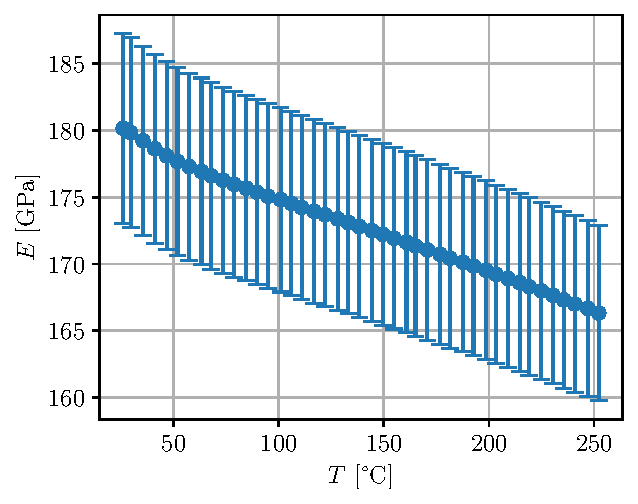
\includegraphics[width=0.6\linewidth]{figures/acier_doux_module_young_temp.pdf}
    \caption{Module de Young d'un échantillon d'acier doux en fonction de la température}
    \label{fig:module_young_temp}
\end{figure}

\paragraph{Frottement intérieur et température} Afin de déterminer plusieurs caractéristiques supplémentaires de l'acier doux des mesures du frottement intérieur en fonction de la température $Q^{-1}(T)$ ont été effectuées. Le pic prédit par l'\autoref{eq:Q_inv_T} à $T_P$ a bien été observé et étudié, il est visible dans


. En raison d'une accumulation d'erreur sur la durée de la mesure, un fit quadratique a été réalisé afin de corriger les valeurs obtenues. Les données brutes ainsi que le fit sont visibles en \autoref{fig:acier_doux_temp_unadjusted}. Le fit de la fonction en \autoref{eq:fit_q1} a été réalisé sur les données corrigées en \autoref{fig:acier_doux_temp_adjusted}. Une valeur de \(\Delta = \textrm{FEUR}\) est alors obtenue.

\begin{figure}[h]
    \centering
    \begin{subfigure}{0.48\linewidth}
        \centering
        % 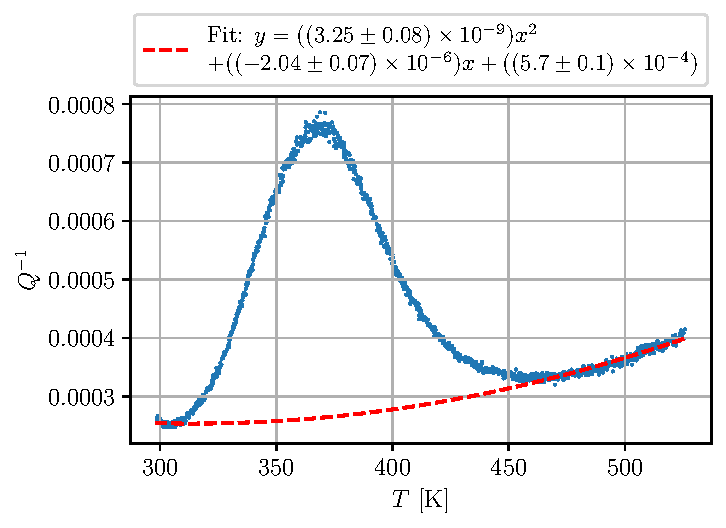
\includegraphics[width=\linewidth]{figures/acier_doux_q_1_temp_unadjusted.pdf}
        \caption{}
        \label{fig:acier_doux_temp_unadjusted}
    \end{subfigure}
    \begin{subfigure}{0.48\linewidth}
        \centering
        % 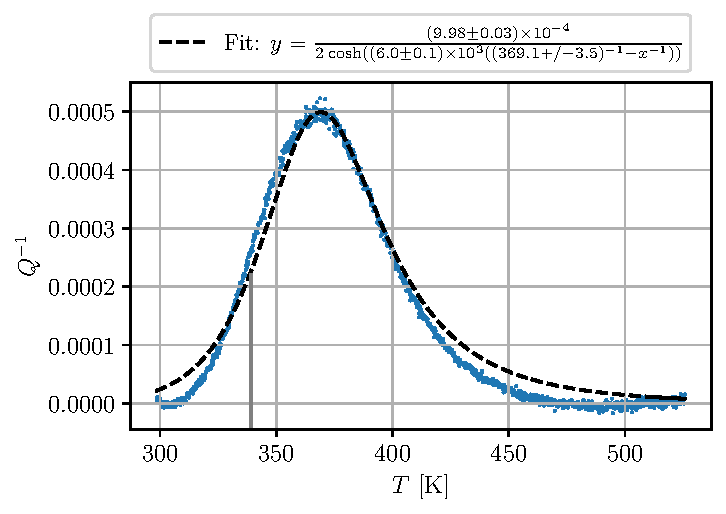
\includegraphics[width=\linewidth]{figures/acier_doux_q_1_temp_adjusted.pdf}
        \caption{}
        \label{fig:acier_doux_temp_adjusted}
    \end{subfigure}
    \caption{Frottement interieur \(Q^{-1}\) pour un échantillon d'acier doux (a) avec l'erreur quadratique (b) sans l'erreur quadratique}
\end{figure}


blabla. Un fit sur la fonction
\begin{equation}
    y(x) = \frac{\Delta}{2 \cosh \left(\frac{H}{k_b}\left(\frac{1}{T_P} - \frac{1}{x}\right)\right)}
    \label{eq:fit_q1}
\end{equation}
où \(H\) est FEUR, \(k_b\) est la constante de Boltzmann, \(T_P\) la température du pic et \(\Delta\) FEUR, qui est la grandeur recherchée

\paragraph{Relaxation anélastique de Snoek}

\paragraph{Concentration de carbone interstitiel}
